\documentclass[12pt]{beamer}
\usepackage{../Estilos/BeamerMAF}
\usepackage{../Estilos/ColoresLatex}
%Sección para el tema de beamer, con el theme, usercolortheme y sección de footers
\usetheme{CambridgeUS}
\usecolortheme{beaver}
%\useoutertheme{default}
\setbeamercovered{invisible}
% or whatever (possibly just delete it)
\setbeamertemplate{section in toc}[sections numbered]
\setbeamertemplate{subsection in toc}[subsections numbered]
\setbeamertemplate{subsection in toc}{\leavevmode\leftskip=3.2em\rlap{\hskip-2em\inserttocsectionnumber.\inserttocsubsectionnumber}\inserttocsubsection\par}
\setbeamercolor{section in toc}{fg=blue}
\setbeamercolor{subsection in toc}{fg=blue}
\setbeamercolor{frametitle}{fg=blue}
\setbeamertemplate{caption}[numbered]

\setbeamertemplate{footline}
\beamertemplatenavigationsymbolsempty
\setbeamertemplate{headline}{}


\makeatletter
\setbeamercolor{section in foot}{bg=gray!30, fg=black!90!orange}
\setbeamercolor{subsection in foot}{bg=blue!30!yellow, fg=red}
\setbeamercolor{date in foot}{bg=black, fg=white}
\setbeamertemplate{footline}
{
  \leavevmode%
  \hbox{%
  \begin{beamercolorbox}[wd=.333333\paperwidth,ht=2.25ex,dp=1ex,center]{section in foot}%
    \usebeamerfont{section in foot} \insertsection
  \end{beamercolorbox}%
  \begin{beamercolorbox}[wd=.333333\paperwidth,ht=2.25ex,dp=1ex,center]{subsection in foot}%
    \usebeamerfont{subsection in foot}  \insertsubsection
  \end{beamercolorbox}%
  \begin{beamercolorbox}[wd=.333333\paperwidth,ht=2.25ex,dp=1ex,right]{date in head/foot}%
    \usebeamerfont{date in head/foot} \insertshortdate{} \hspace*{2em}
    \insertframenumber{} / \inserttotalframenumber \hspace*{2ex} 
  \end{beamercolorbox}}%
  \vskip0pt%
}
\makeatother\newlength{\depthofsumsign}
\setlength{\depthofsumsign}{\depthof{$\sum$}}
\newcommand{\nsum}[1][1.4]{% only for \displaystyle
    \mathop{%
        \raisebox
            {-#1\depthofsumsign+1\depthofsumsign}
            {\scalebox
                {#1}
                {$\displaystyle\sum$}%
            }
    }
}
\def\scaleint#1{\vcenter{\hbox{\scaleto[3ex]{\displaystyle\int}{#1}}}}
\def\bs{\mkern-12mu}






\date{}

\title{\large{Ecuaciones Diferenciales Parciales}}
\subtitle{Tema 2 - Primeras técnicas de solución}
\author{M. en C. Gustavo Contreras Mayén}

\begin{document}
\maketitle
\fontsize{14}{14}\selectfont
\spanishdecimal{.}

\section*{Contenido}
\frame{\tableofcontents[currentsection, hideallsubsections]}

\section{Condiciones de frontera e iniciales}
\frame{\tableofcontents[currentsection, hideothersubsections]}
\subsection{Características de la EDP}

\begin{frame}
\frametitle{Obteniendo soluciones}
Una vez que se ha realizado la formulación de una EDP el siguiente paso es resolver la ecuación, en un primer momento podemos considerar la solución general de la EDP, entonces en vez de constantes arbitrarias aparecen funciones arbitrarias.
\end{frame}
\begin{frame}
\frametitle{Obteniendo soluciones}
Por ejemplo, la solución general de $u_{xy} = 0$ es :
\pause
\begin{align*}
u (x, y) = G (x) + F (y)
\end{align*}
donde $G$, $F$ son funciones arbitrarias.
\end{frame}

\begin{frame}
\frametitle{Unicidad de la solución}
Dado que se quieren resolver problemas específicos, hay que estudiar el tipo de condiciones que hay que imponer para garantizar \emph{la unicidad} de la solución.
\end{frame}
\begin{frame}
\frametitle{Unicidad de la solución}
Como se revisó en la presentación anterior, tenemos una clasificación con tres tipos de ecuaciones (parabólica, hiperbólica y elíptica) a continuación presentamos un posible tipo de condiciones de frontera (CDF) que se pueden presentar.
\end{frame}

\subsection{Condiciones para una EDP Parabólica}

\begin{frame}
\frametitle{Condiciones para una EDP parabólica}
Consideremos la ecuación del calor:
\pause
\begin{align*}
u_{t} =  \alpha^{2} \,  u_{xx}
\end{align*}
En este caso se trabajará con un problema unidimensional, es decir, la transmisión del calor a lo largo de una barra de longitud $L$.
\end{frame}
\begin{frame}
\frametitle{Condición inicial para una EDP Parabólica}
Para que el problema tenga solución se debe de especificar la distribución inicial de temperatura de la barra, es decir, hay que dar una función $\varphi (x)$ de modo que:
\pause
\begin{align}
u (x, 0) = \alpha (x) \hspace{1.5cm} 
\label{eq:ecuacion_06_02_02}
\end{align}
sería una distribución inicial de temperatura. \pause En analogía con las EDO, tiene sentido llamar tal condición una \textocolor{red}{condición inicial}.
\end{frame}
\begin{frame}
\frametitle{Condiciones de frontera para una EDP Parabólica}
A su vez, como la barra tiene una longitud finita, hay que especificar la interacción de los extremos de la barra con el medio ambiente.
\\
\bigskip
\pause
Tales condiciones se conocen como \textocolor{blue}{condiciones de frontera}.
\end{frame}
\begin{frame}
\frametitle{Tipos de condición para una EDP Parabólica}
Para los problemas de una dimensión hay tres tipos de condiciones de frontera usuales, aunque solo se estudiarán las primeras dos en esta revisión:
\setbeamercolor{item projected}{bg=oxfordblue,fg=paleaqua}
\setbeamertemplate{enumerate items}{%
\usebeamercolor[bg]{item projected}%
\raisebox{1.5pt}{\colorbox{bg}{\color{fg}\footnotesize\insertenumlabel}}%
}
\begin{enumerate}[<+->]
\item \textocolor{palatinatepurple}{Condición de Dirichlet}: Consiste en especificar la temperatura en los extremos de la barra en todo instante, es decir, dar dos funciones $f(t)$ y $g(t)$ de modo que:
\begin{align}
u(0, t) = f (t)  \hspace{1cm} u(L, t) = g(t)
\label{eq:ecuacion_06_02_03}    
\end{align}
\seti
\end{enumerate}
\end{frame}
\begin{frame}
\frametitle{Tipos de condición para una EDP Parabólica}
\setbeamercolor{item projected}{bg=oxfordblue,fg=paleaqua}
\setbeamertemplate{enumerate items}{%
\usebeamercolor[bg]{item projected}%
\raisebox{1.5pt}{\colorbox{bg}{\color{fg}\footnotesize\insertenumlabel}}%
}
\begin{enumerate}[<+->]
\conti
\item \textocolor{persianblue}{Condición de Neumann}: Consiste en especificar la derivada de la temperatura en los extremos de la barra, es decir, especificar el flujo de calor en los extremos de la barra:
\begin{align}
u_{x}(0,t) = f(t) \hspace{1cm} u_{x}(L,t) = g(t)
\label{eq:ecuacion_06_02_04}    
\end{align}
\seti
\end{enumerate}
\end{frame}
\begin{frame}
\frametitle{Tipos de condición para una EDP Parabólica}
\setbeamercolor{item projected}{bg=oxfordblue,fg=paleaqua}
\setbeamertemplate{enumerate items}{%
\usebeamercolor[bg]{item projected}%
\raisebox{1.5pt}{\colorbox{bg}{\color{fg}\footnotesize\insertenumlabel}}%
}
\begin{enumerate}[<+->]
\conti
\item \textocolor{persianplum}{Condiciones mixtas (de Robin)}: Consiste en especificar una combinación de $u$ y de $u_{x}$ en los extremos de la barra.
\end{enumerate}
\end{frame}

\subsection{Condiciones para una EDP Elíptica}

\begin{frame}
\frametitle{Una EDP elíptica}
Sea la ecuación de Laplace:
\pause
\begin{align*}
u_{xx} + u_{yy} = 0
\end{align*}
\\
\bigskip
\pause
Se puede interpretar como la ecuación de un potencial electrostático sobre una región del plano $xy$ o bien la distribución de temperatura en el caso estacionario para una placa o una región del plano $xy$.
\end{frame}
\begin{frame}
\frametitle{Tipos de condición para una EDP elíptica}
En este caso no hay que especificar condiciones iniciales pues la función no depende del tiempo.
\end{frame}
\begin{frame}
\frametitle{Tipos de condición para una EDP elíptica}
Se estudiarán dos tipos de condiciones:
\setbeamercolor{item projected}{bg=pink,fg=black}
\setbeamertemplate{enumerate items}{%
\usebeamercolor[bg]{item projected}%
\raisebox{1.5pt}{\colorbox{bg}{\color{fg}\footnotesize\insertenumlabel}}%
}
\begin{enumerate}[<+->]
\item \textocolor{prune}{Condición de Dirichlet}: Si se trabaja sobre una lámina rectangular $0 < x < a$ y $0 < y < b$ las condiciones de Dirichlet consisten en especificar los valores de la temperatura (o el potencial) sobre todos los lados, es decir:
\begin{align}
\begin{aligned}
u (0, y) &= f_{1} (y) \hspace{1.5cm} u (a, y) = f_{2} (y) \\
u (x, 0) &= g_{1} (x) \hspace{1.5cm} u (x, b) = g_{2} (x)
\end{aligned}
\label{eq:ecuacion_06_02_05}
\end{align}
\seti
\end{enumerate}
\end{frame}
\begin{frame}
\frametitle{Tipos de condición para una EDP elíptica}
\setbeamercolor{item projected}{bg=pink,fg=black}
\setbeamertemplate{enumerate items}{%
\usebeamercolor[bg]{item projected}%
\raisebox{1.5pt}{\colorbox{bg}{\color{fg}\footnotesize\insertenumlabel}}%
}
\begin{enumerate}[<+->]
\conti
\item \textocolor{prussianblue}{Condiciones Mixtas}: Para los lados de la placa se toman dos de las condiciones de Dirichlet y las otras dos de Neumann, por ejemplo:
\begin{align}
\begin{aligned}
u_{y} (0, y) &= f_{1} (y) \hspace{1.5cm} u_{y} (a, y) = f_{2} (y) \\
u (x, 0) &= g_{1} (x) \hspace{1.5cm} u (x, b) = g_{2} (x)
\end{aligned}
\label{eq:ecuacion_06_01_06}
\end{align}
\end{enumerate}
\end{frame}

\subsection{Condiciones para una EDP Hiperbólica}

\begin{frame}
\frametitle{Una EDP hiperbólica}
La ecuación de onda:
\pause
\begin{align*}
u_{tt} = v^{2} \, u_{xx}
\end{align*}
\\
\bigskip
\pause
En este caso se considera una cuerda de longitud $L$.
\end{frame}
\begin{frame}
\frametitle{Condiciones para una EDP hiperbólica}
Como la ecuación es de segundo orden en el tiempo, tiene sentido esperar que haya que especificar la posición inicial de la cuerda así como su velocidad inicial, es decir, proporcionar las \textocolor{regalia}{condiciones iniciales}:
\pause
\begin{align}
u (x, 0) = \phi (x) \hspace{1.5cm} u_{t} (x, 0) = \psi (x)
\label{eq:ecuacion_06_02_07}
\end{align}
\end{frame}
\begin{frame}
\frametitle{Condiones para una EDP hiperbólica}
A su vez, hay que especificar como se relaciona la cuerda con su frontera y nuevamente se van a estudiar las condiciones de Dirichlet y de Neumann.
\pause
\setbeamercolor{item projected}{bg=bananayellow,fg=blue}
\setbeamertemplate{enumerate items}{%
\usebeamercolor[bg]{item projected}%
\raisebox{1.5pt}{\colorbox{bg}{\color{fg}\footnotesize\insertenumlabel}}%
}
\begin{enumerate}[<+->]
\item \textocolor{richblack}{Condición de Dirichlet}: Se especifica la posición de los extremos de la cuerda, es decir:
\begin{align}
u(0, t) = f (t) \hspace{1.5cm} u(L, t) = g(t)
\label{eq:ecuacion_06_02_08}   
\end{align}
\seti
\end{enumerate}
\end{frame}
\begin{frame}
\frametitle{Condiones para una EDP hiperbólica}
\setbeamercolor{item projected}{bg=bananayellow,fg=blue}
\setbeamertemplate{enumerate items}{%
\usebeamercolor[bg]{item projected}%
\raisebox{1.5pt}{\colorbox{bg}{\color{fg}\footnotesize\insertenumlabel}}%
}
\begin{enumerate}[<+->]
\conti    
\item \textocolor{rosewood}{Condición de Neumann}: Se especifica la forma en que se están \enquote{jalando} los extremos de la cuerda, es decir:
\begin{align}
u_{x} (0, t) = f (t) \hspace{1.5cm} u_{x} (L, t) = g (t)
\label{eq:ecuacion_06_02_09}    
\end{align}
\end{enumerate}
\end{frame}

\section{Condición para separar variables}
\frame{\tableofcontents[currentsection, hideothersubsections]}
\subsection{Separación de variables}

\begin{frame}
\frametitle{Suposición importante}
Como se veremos más adelante, el \textocolor{sangria}{método de separación de variables} consiste en suponer que la solución depende como un producto de funciones, cada una de las cuales depende exclusivamente de una de las variables independientes.
\end{frame}
\begin{frame}
\frametitle{Condiciones de frontera}
Para que tenga éxito el método, se ocupará que varias de las condiciones de frontera estén igualadas a cero, de forma que se utilicen para restringir las soluciones a las ecuaciones diferenciales ordinarias que aparecen.
\end{frame}
\begin{frame}
\frametitle{Principio de superposición}
Luego, dado que las ecuaciones son lineales se propone por el principio de superposición una combinación lineal (de hecho una serie en la mayoría de los casos) de tales soluciones y las constantes que aparecen se hallan tomando el desarrollo de Fourier de las otras condiciones iniciales o de frontera que todavía no se han utilizado.
\end{frame}

\section{Método de separación de variables}
\frame[allowframebreaks]{\tableofcontents[currentsection, hideothersubsections]}
\subsection{La técnica}

\begin{frame}
\frametitle{Separación de variables}
El método de separación de variables es una de las técnicas más antiguas para resolver problemas de valores con condiciones iniciales y se aplica en problemas donde:
\pause
\setbeamercolor{item projected}{bg=sealbrown,fg=seashell}
\setbeamertemplate{enumerate items}{%
\usebeamercolor[bg]{item projected}%
\raisebox{1.5pt}{\colorbox{bg}{\color{fg}\footnotesize\insertenumlabel}}%
}
\begin{enumerate}[<+->]
\item La EDP es lineal y homogénea (no necesariamente con coeficientes constantes).
\seti
\end{enumerate}
\end{frame}
\begin{frame}
\frametitle{Separación de variables}
\setbeamercolor{item projected}{bg=sealbrown,fg=seashell}
\setbeamertemplate{enumerate items}{%
\usebeamercolor[bg]{item projected}%
\raisebox{1.5pt}{\colorbox{bg}{\color{fg}\footnotesize\insertenumlabel}}%
}
\begin{enumerate}[<+->]
\conti    
\item Las condiciones de frontera tienen la forma:
\begin{align*}
\alpha \, u_{x} (0, t) + \beta \, u (0, t) &= 0 \\
\gamma \, u_{x} (1, t) + \delta \, u (1, t) &= 0
\end{align*}
donde $\alpha, \beta, \gamma, \delta$ son constantes (las condiciones de frontera de esta forma se denominan \textocolor{sienna}{condiciones de frontera lineales homogéneas}).
\end{enumerate}
\end{frame}
\begin{frame}
\frametitle{La técnica de separación de variables}
Como referencia histórica, este método se remonta a la época de Joseph Fourier (de hecho, ocasionalmente se le llama \textbf{método de Fourier}) y es probablemente el método de solución más utilizado (cuando corresponde).
\end{frame}
\begin{frame}
\frametitle{Practicando la técnica}
En lugar de mostrar cómo funciona el método en general, apliquémoslo a un problema específico.
\\
\bigskip
\pause
El procedimiento se debe de realizar de la misma manera cuando tengamos que resolver un problema mediante esta técnica.
\end{frame}

\subsection{Planteamiento del problema}

\begin{frame}
\frametitle{El problema a resolver}
Considera el siguiente problema de valores iniciales con la ecuación de calor:
\\
\bigskip
\pause
Ecuación diferencial:
\begin{align*}
\addtolength{\fboxsep}{5pt}\boxed{ u_{t} = \alpha^{2} \, u_{xx}, \hspace{1.5cm} 0 < x < L,\hspace{0.5cm} 0 < t < \infty}
\end{align*}
\end{frame}
\begin{frame}
\frametitle{CDF del problema}
Condiciones de frontera (CDF):
\pause
\begin{align*}
\addtolength{\fboxsep}{5pt}\boxed{
\begin{cases}
u (0, t) = 0 \\
u (L, t) = 0
\end{cases}
\hspace{1.5cm}
0 < t < \infty }
\end{align*}
\end{frame}
\begin{frame}
\frametitle{Condiciones iniciales del problema}
Condiciones iniciales (CI):
\pause
\begin{align*}
\addtolength{\fboxsep}{5pt}\boxed{
u (x, 0) = \phi (x) \hspace{1.5cm} 0 \leq x \leq L
}
\end{align*}
\end{frame}
\begin{frame}
\frametitle{Recomendación previa}
Antes de revisar el método de separación de variables, pensemos primero en nuestro problema: \pause Aquí tenemos una varilla finita de longitud $L$ donde la temperatura en los extremos se fija en cero (supongamos que es un problema de temperatura donde cero significa tantos grados).
\end{frame}
\begin{frame}
\frametitle{Esquema del problema}
\begin{figure}[H]
    \centering
    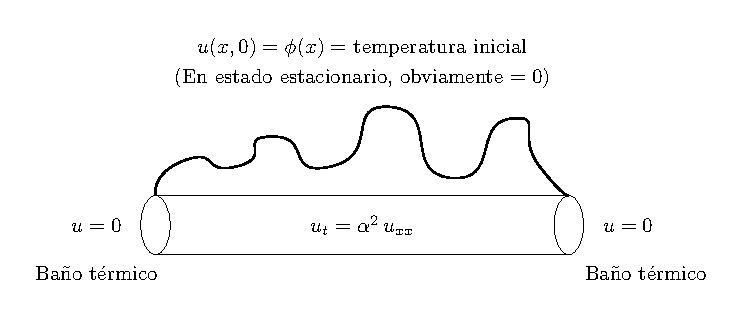
\includegraphics[scale=0.9]{Imagenes/Separacion_Variables_00_Barra.eps}
    \caption{Esquema que representa la barra conductora así como las condiciones iniciales y de frontera.}
    \label{fig:figura_barra_01}
\end{figure}
\end{frame}
\begin{frame}
\frametitle{Revisando previamente el problema}
También se nos dan datos sobre el problema en forma de condición inicial.
\\
\bigskip
\pause
Nuestro objetivo es encontrar la temperatura $u (x, t)$ en valores posteriores al tiempo inicial.
\end{frame}

\subsection{La técnica de separación de variables}

\begin{frame}
\frametitle{Suposición inicial}
El método de separación de variables \textocolor{ao}{supone la existencia de soluciones sencillas} de una EDP de la forma:
\pause
\begin{align*}
u (x, t) =  X (x) \, T (t)
\end{align*}
\pause
donde $X (x)$ es alguna \textocolor{lava}{función que depende solo de} $x$ \pause y $T (t)$ es alguna \textocolor{armygreen}{función que depende solo de} $t$.
\end{frame}
\begin{frame}
\frametitle{El por qué de las soluciones sencillas}
Las soluciones son sencillas porque cualquier temperatura $u (x, t)$ de esta forma conservará su \textbf{forma} básica para diferentes valores de tiempo $t$, como podemos ver en la figura (\ref{fig:figura_separacion_variables_01})
\end{frame}
\begin{frame}
\frametitle{Esquema de las soluciones sencillas}
\begin{figure}[H]
    \centering
    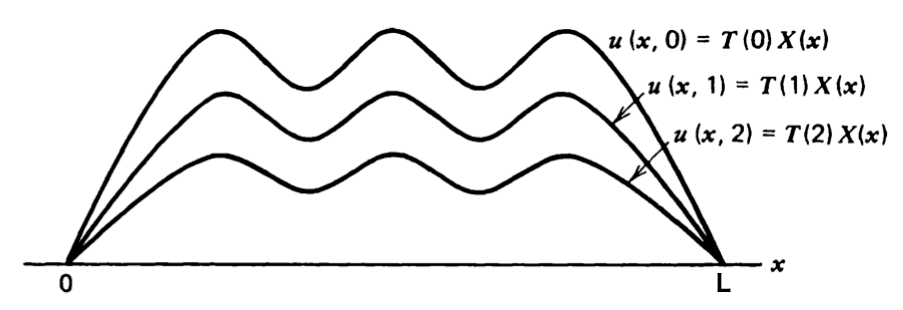
\includegraphics[scale=0.35]{Imagenes/Separacion_Variables_01.png}
    \caption{Gráfica de $X (x)$ y $T (t)$ para distintos valores de $t$.}
    \label{fig:figura_separacion_variables_01}
\end{figure}
\end{frame}
\begin{frame}
\frametitle{Acotando las soluciones}
La idea general que tenemos nos plantea la posibilidad de encontrar un número infinito de estas soluciones a la EDP (que al mismo tiempo también satisfacen las condiciones de frontera).
\end{frame}
\begin{frame}
\frametitle{Las funciones sencillas}
A estas funciones sencillas:
\pause
\begin{align*}
u_{n} (t) = X_{n} (x) \, T_{n} (t)
\end{align*}
\pause
se les denomina \textocolor{teal}{soluciones fundamentales}, son las componentes básicas de nuestro problema, y de la solución $u (x, t)$ que estamos buscando.
\end{frame}
\begin{frame}
\frametitle{Sumando soluciones fundamentales}
Sumando las soluciones fundamentales $X_{n} (x) \, T_{n} (t)$ de tal manera que la suma resultante:
\pause
\begin{align*}
\nsum_{n=1}^{\infty} A_{n} \, X_{n} (x) \, T_{n} (t)
\end{align*}
\pause
satisface las condiciones iniciales. \pause Dado que esta suma aún satisface la EDP y las CDF, ahora tenemos la solución a nuestro problema. Veamos a detalle el método de separación de variables.
\end{frame}

\subsection{Paso 1}

\begin{frame}
\frametitle{Paso 1 - Soluciones elementales}
\textbf{Encontrar las soluciones elementales de la EDP.}
\pause
Nos interesa encontrar la función $u (x, t)$ que satisfaga las siguientes condiciones:
\pause
\begin{align*}
\mbox{EDP} \hspace{1.5cm} &u_{t} = \alpha^{2} \, u_{xx} \hspace{1cm} 0 < x < L, \hspace{0.3cm} 0 < t < \infty \\[0.5em] 
\mbox{CDF} \hspace{1.5cm} &\begin{cases}
    u (0, t) = 0 \\
    u (L, t) = 0
    \end{cases}
    \hspace{1cm}
    0 < t < \infty \\[0.5em]
\mbox{CI} \hspace{1.5cm} & u (x, 0) = \phi (x) \hspace{1cm} 0 \leq x \leq L
\end{align*}
\end{frame}
\begin{frame}
\frametitle{Propuesta de solución}
Para comenzar, buscamos soluciones de la forma $u (x, t) = X(x) \, T (t)$ sustituyendo $X (x) \, T (t)$ en la EDP y resolvemos para  $X (x) \, T (t)$.
\\
\bigskip
\pause
Haciendo esta sustitución obtenemos:
\pause
\begin{align*}
X (x) \, \pderivada{T} (t) = \alpha^{2} \, \sderivada{X} (x) \, T (t)
\end{align*}
\end{frame}
\begin{frame}
\frametitle{Avanzando en el paso}
La parte que hace todo el trabajo es la siguiente: si \emph{dividimos} cada lado de esta ecuación por $\alpha^{2} \, X (x) \, T (t)$, tenemos que:
\pause
\begin{align*}
\dfrac{\pderivada{T} (t)}{\alpha^{2} \, T (t)} = \dfrac{\sderivada{X} (x)}{X (x)}
\end{align*}
\end{frame}
\begin{frame}
\frametitle{Variables separables}
Para obtener lo que se conoce como \textocolor{blue}{variables separables}, es decir, la expresión del lado izquierdo de la igualdad depende solo de $t$, mientras que la expresión del lado derecho\footnote{El primado sencillo indica la diferenciación de primer grado con respecto a la variable señalada, mientras que el primado doble, señala la diferenciación de segundo grado con respecto a la variable que se indica.}, depende solo de $x$.
\end{frame}
\begin{frame}
\frametitle{Variables independientes}
Dado que $x$ y $t$ son independientes entre sí, cada lado debe ser una constante fija (digamos $k$),  por tanto podemos escribir:
\pause
\begin{align*}
\dfrac{\pderivada{T}}{\alpha^{2} \, T} = \dfrac{\sderivada{X}}{X} = k
\end{align*}
\end{frame}
\begin{frame}
\frametitle{Variables independientes}
De manera equivalente:
\pause
\begin{align*}
\pderivada{T} - k \, \alpha^{2} \, T &= 0 \\[0.5em]
\sderivada{X} - k \, X &= 0
\end{align*}
\pause
Entonces, ahora podemos resolver cada uno de estas dos EDO, para luego multiplicarlas y así obtener una solución a la EDP (toma en cuenta que esencialmente hemos cambiado una EDP de segundo orden a dos EDO)
\end{frame}
\begin{frame}
\frametitle{La constante de separación}
Sin embargo, ahora hacemos una observación importante, a saber, queremos que la constante de separación $k$ sea negativa (o de lo contrario el factor $T (t)$ no se anula cuando $t \to \infty$).
\\
\bigskip
\pause
Teniendo esto en cuenta, es una práctica general cambiar el nombre de $k = - \lambda$, donde $\lambda$ es distinta de cero. 
\end{frame}
\begin{frame}
\frametitle{La constante de separación}
Llamando a nuestra \textocolor{ultramarine}{constante de separación} por su nuevo nombre, ahora podemos escribir las dos EDO como:
\begin{align*}
\pderivada{T} + \lambda \, \alpha^{2} \, T &= 0 \\[0.5em]
\sderivada{X} + \lambda \, X &= 0
\end{align*}
\pause
Ahora podemos resolver ese par de ecuaciones.
\end{frame}
\begin{frame}
\frametitle{Resolviendo las EDO}
Para $\sderivada{X} + \lambda \, X = 0$, las soluciones son de la forma:
\pause
\begin{align}
\begin{cases}
X (x) = A + B \, x & \hspace{0.2cm} \lambda = 0 \\
X (x) = A \, e^{a x} + B \, e^{-a x} & \hspace{0.2cm} \lambda = - a^{2} \\
X (x) = A \cos (a x ) + B \, \sin (a x) & \hspace{0.2cm} \lambda = a^{2}
\end{cases}
\label{eq:ecuacion_06_02_31}
\end{align}
\end{frame}
\begin{frame}
\frametitle{Resolviendo las EDO}
Mientras que para $\pderivada{T} + \lambda \, \alpha^{2} \, T = 0$ se tiene:
\pause
\begin{align}
T (t) = A \, e^{- \lambda \, \alpha^{2} \, t} \hspace{1.5cm} \mbox{con A arbitraria}
\label{eq:ecuacion_06_02_36a}    
\end{align}
y de aquí
\begin{align*}
u (x, t) = X (x) \, T (t) 
\end{align*}
\pause
En este punto, tenemos un número infinito de funciones que satisfacen la EDP.
\end{frame}

\subsection{Paso 2}

\begin{frame}
\frametitle{Paso 2 - Soluciones con las CDF}
\textbf{Encontrar las soluciones de la EDP con las CDF.}
\pause
Ahora debemos de considerar un subconjunto de las soluciones obtenidas en el paso anterior, que a su vez satisfagan las condiciones de frontera (CDF):
\pause
\begin{align*}
u (0, t) &= 0 \\[0.5em]
u (L, t) &= 0
\end{align*}
\end{frame}
\begin{frame}
\frametitle{Soluciones con las CDF}
Por las CDF, únicamente en las posibles soluciones para $X(x)$ (ec. \ref{eq:ecuacion_06_02_31}), la tercera posibilidad produce una solución no trivial:
\pause
\begin{align*}
X (x) = A \cos (a x ) + B \, \sin (a x), & \hspace{0.2cm} \lambda = a^{2}
\end{align*}
\end{frame}
\begin{frame}
\frametitle{Soluciones con las CDF}
De hecho, trabajando con:
\pause
\begin{align*}
X (x) = A \cos (a x) + B \, \sin (a x) \hspace{2cm}
\end{align*}
\pause
que al sustituir en la solución, multiplicando la solución de $X (t)$ y de $T (t)$:
\begin{eqnarray*}
u (0, t) &=& A \, e^{-\lambda \alpha^{2} \, t} = 0 \pause \hspace{0.3cm} \Longrightarrow \hspace{0.3cm} A = 0 \\[0.5em] \pause
u (L, t) &=& B \, e^{-\lambda \alpha^{2} \, t} \, \sin (\lambda \, L) = 0 \pause \hspace{0.3cm} \Longrightarrow \hspace{0.3cm} \sin (\lambda \, L) = 0
\end{eqnarray*}
\end{frame}
\begin{frame}
\frametitle{Restricción en la constante de separación}
Esta última CDF restringe la constante de separación $\lambda$ de ser cualquier número distinto de cero, debe ser una raíz de la ecuación $\sin (\lambda \, L) = 0$.
\\
\bigskip
\pause
En otras palabras, para que $u (L, t) = 0$, es necesario elegir:
\pause
\begin{align}
\lambda \, L = n \, \pi \hspace{1.5cm} n \in \mathbb{Z}
\label{eq:ecuacion_06_02_34}    
\end{align}
\end{frame}
\begin{frame}
\frametitle{Conjunto infinito de soluciones}
Sin embargo, para no contar dos veces la misma solución, se toma $n$ positivo, es decir:
\pause
\begin{align}
\lambda = \dfrac{n^{2} \, \pi^{2}}{L^{2}} \hspace{1.5cm} n = 1, 2, 3, \ldots
\label{eq:ecuacion_06_02_35}
\end{align}
\pause
En este paso hemos encontrado un número infinito de funciones que son solución a la EDP:
\pause
\begin{align}
u_{n} (x, t) = A_{n} \, \exp \left( - \dfrac{n^{2} \, \alpha^{2} \, \pi^{2}}{L^{2}} \, t \right) \, \sin \left( \dfrac{n \, \pi}{L} \, x \right)
\label{eq:ecuacion_06_02_37}    
\end{align}
\end{frame}
\begin{frame}
\frametitle{Usando el principio de superposición}
Por el principio de superposición, la solución que se propone es:
\pause
\begin{align}
u (x, t) = \nsum_{n=1}^{\infty} A_{n} \, \exp \left( - \dfrac{n^{2} \, \alpha^{2} \, \pi^{2}}{L^{2}} \, t \right) \, \sin \left( \dfrac{n \, \pi}{L} \, x \right)
\label{eq:ecuacion_06_02_38}
\end{align}
\pause
Nos queda por considerar las condiciones iniciales del problema para obtener entonces la solución a la EDP.
\end{frame}

\subsection{Paso 3}

\begin{frame}
\frametitle{Paso 3 - Solución con la CI}
\textbf{Encontrar la solución de la EDP, con las CDF y la condición inicial.}
\\
\bigskip
\pause
El último paso (y probablemente el más interesante desde un punto de vista matemático) es agregar las soluciones fundamentales (ec. \ref{eq:ecuacion_06_02_38}) de tal manera (eligiendo los coeficientes $A_{n}$) que la condición inicial:
\pause
\begin{align*}
u (x, 0) = \phi (x)
\end{align*}
se satisfaga.
\end{frame}
\begin{frame}
\frametitle{Usando la CI}
Utilizando la CI en la suma, se tiene que:
\pause
\begin{align*}
\phi (x) = \nsum_{n=1}^{\infty} A_{n} \, \sin \left( \dfrac{n \, \pi}{L} \, x \right)
\end{align*}
\pause
Vemos que esto es equivalente a encontrar el desarrollo en series de la función seno de $\phi (x)$.
\end{frame}
\begin{frame}
\frametitle{Solución en series}
Se debe de ocupar el desarrollo en una serie de Fourier y ocupar la propiedad de ortogonalidad de la función seno.
\\
\bigskip
\pause
Por lo que:
\begin{align}
A_{n} = \dfrac{2}{L} \scaleint{6ex}_{\bs 0}^{L} \phi (x) \, \sin \left( \dfrac{n \, \pi}{L} \, x \right) \dd{x}
\label{eq:ecuacion_06_02_40}    
\end{align}
\end{frame}
\begin{frame}
\frametitle{Solución completa al problema}
Entonces la solución completa al problema de Dirichlet para la ecuación de calor es:
\pause
\begin{align*}
u (x, t) &= \dfrac{2}{L} \nsum_{n=1}^{\infty} \left[ \scaleint{6ex}_{\bs 0}^{L} \phi (x) \, \sin \left( \dfrac{n \, \pi}{L} \, x \right) \dd{x} \right] \times \\[1em]
&\times \exp \left( - \dfrac{n^{2} \, \alpha^{2} \, \pi^{2}}{L^{2}} \, t \right) \, \sin \left( \dfrac{n \, \pi}{L} \, x \right)
\end{align*}
\end{frame}

\section{Enunciado}
\frame{\tableofcontents[currentsection, hideothersubsections]}
\subsection{El ejercicio a resolver}

\begin{frame}
\frametitle{El problema}
Demostrar que la ecuación de Helmholtz:
\begin{align*}
\laplacian{\psi} + k^{2} \, \psi = 0
\end{align*}
\emph{es separable} en coordenadas cilíndricas circulares, \pause si $k^{2}$ se generaliza como:
\pause
\begin{align*}
k^{2} + f(\rho) + \left( \dfrac{1}{\rho^{2}} \right) \, g(\varphi) + h(z)
\end{align*}
\end{frame}
\begin{frame}
\frametitle{Reexpresando la ecuación}
La ecuación que debemos de demostrar que es separable es:
\begin{align*}
\laplacian{\psi} + \left[ k^{2} + f(\rho) + \left( \dfrac{1}{\rho^{2}} \right) \, g(\varphi) + h(z) \right] \, \psi = 0
\end{align*}
\pause
Debemos de utilizar el operador laplaciano en el sistema de coordenadas cilíndricas circulares.
\end{frame}
\begin{frame}
\frametitle{Ocupando lo que ya conocemos}
Recordemos que tenemos una expresión que nos determina el operador diferencial laplaciano en términos de un sistema de coordenadas generalizado.
\\
\bigskip
\pause
Será necesario contar con las reglas de transformación así como de los factores de escala de ese sistema, para obtener el operador, todo esto lo recuperamos del Tema 1.
\end{frame}
\begin{frame}
\frametitle{La ecuación en el sistema cilíndrico}
Tenemos entonces que la expresión resulta ser:
\pause
\begin{align*}
&{} \dfrac{1}{\rho} \, \pdv{\rho} \left( \rho \, \pdv{\psi}{\rho} \right) + \dfrac{1}{\rho^{2}} \, \pdv[2]{\psi}{\varphi} + \pdv[2]{\psi}{z} + \\[1em]
&+ \left[ k^{2} + f(\rho) + \left( \dfrac{1}{\rho^{2}} \right) \, g(\varphi) + h(z) \right] \, \psi = 0
\end{align*}
\end{frame}

\section{Resolviendo el problema}
\frame[allowframebreaks]{\tableofcontents[currentsection, hideothersubsections]}
\subsection{Propuesta de solución}

\begin{frame}
\frametitle{Proponemos una solución}
Para aplicar el método de separación de variables, proponemos la siguiente solución:
\begin{align*}
\psi (\rho, \varphi, z) = R(\rho) \, \Phi (\varphi) \, Z(z)
\end{align*}
\pause
donde cada función con letra mayúscula, depende de una sola variable.
\end{frame}

\subsection{Obteniendo las derivadas}

\begin{frame}
\frametitle{Obteniendo las derivadas}
Como ya propusimos una solución, ahora hay que calcular las derivadas parciales y sustituirlas en la ecuación de Helmholtz.
\\
\bigskip
\pause
Haremos en este ejercicio el procedimiento de diferenciación.
\end{frame}
\begin{frame}
\frametitle{Calculando las derivadas}
Comenzamos con las derivadas parciales con respecto a $\rho$:
\pause
\begin{eqnarray*}
\rho \, \pdv{\psi}{\rho} = \pause \rho \, \pdv{\rho} R(\rho) \Phi (\varphi) Z(z) = \pause \rho \left( \ptilde{R} \, \Phi Z \, \right)
\end{eqnarray*}
\pause
Notemos que:
\setbeamercolor{item projected}{bg=blue!70!black,fg=yellow}
\setbeamertemplate{enumerate items}[circle]
\begin{enumerate}[<+->]
\item Cada función con mayúsculas depende de una sola variable.
\item El primado indica que tenemos una derivada ordinaria de la función con respecto a su variable.
\end{enumerate}
\end{frame}
\begin{frame}
\frametitle{Continuamos derivando con respecto a $\rho$}
La siguiente derivada parcial es:
\begin{align*}
\dfrac{1}{\rho} \pdv{\rho} \left( \rho \, \pdv{\psi}{\rho}  \right) = \pause \stilde{R} \, \Phi \, Z + \dfrac{1}{\rho} \, \ptilde{R} \, \Phi \, Z
\end{align*}
\\
\bigskip
\pause
Ya concluimos las diferenciaciones con respecto a $\rho$, por lo que podemos continuar con las otras dos variables.
\end{frame}
\begin{frame}
\frametitle{Las otras dos derivadas}
Tendremos entonces:
\begin{eqnarray*}
\dfrac{1}{\rho^{2}} \, \pdv[2]{\psi}{\varphi} &=& \pause \dfrac{1}{\rho^{2}} \, \pdv[2]{\varphi} \, R(\rho) \Phi (\varphi) Z(z) = \pause \dfrac{1}{\rho^{2}} \, R \, \stilde{\Phi} \, Z \\[1em] \pause
\pdv[2]{\psi}{z} &=& \pause \pdv[2]{z} \, R(\rho) \Phi (\varphi) Z(z) = \pause R \, \Phi \, \stilde{Z}
\end{eqnarray*}
\end{frame}
\begin{frame}
\frametitle{Juntado los elementos en la ecuación}
Al incluir las derivadas que hemos obtenido, la ecuación resulta ser:
\begin{align*}
&{} \stilde{R} \, \Phi \, Z + \dfrac{1}{\rho} \, \ptilde{R} \, \Phi \, Z + \dfrac{1}{\rho^{2}} R \, \stilde{\Phi} \, Z + R \, \Phi \, \stilde{Z} + \\[1em]
&+ \left[ k^{2} + f(\rho) + \left( \dfrac{1}{\rho^{2}} \right) \, g(\varphi) + h(z) \right] \, R \, \Phi \, Z = 0
\end{align*}
\end{frame}

\subsection{Siguiente paso: dividir entre la solución}

\begin{frame}
\frametitle{El siguiente paso}
El paso que debemos de realizar es: dividir toda la expresión entre la solución propuesta, es decir, entre: $R \, \Phi \, Z$, por lo que tenemos:
\pause
\begin{align*}
&{} \dfrac{1}{R} \left( \stilde{R} + \dfrac{1}{\rho} \, \ptilde{R} \right) + \dfrac{1}{\rho^{2}} \, \dfrac{\stilde{\Phi}}{\Phi} + \dfrac{\stilde{Z}}{Z} + \\[1em]
&+ k^{2} + f(\rho) + \left( \dfrac{1}{\rho^{2}} \right) \, g(\varphi) + h(z) = 0    
\end{align*}
\end{frame}

\subsection{Constantes de separación}

\begin{frame}
\frametitle{Reacomodando los términos}
Procedemos a reacomodar los términos por cada una de las variables, buscando que haya una dependencia en una sola de ellas en la expresión.
\\
\bigskip
\pause
Veamos lo qué pasa cuando pasamos los términos que involucran a la variable $z$ al lado derecho de la expresión.
\end{frame}
\begin{frame}
\frametitle{La expresión separada}
Entonces vemos que:
\pause
\begin{align*}
&{} \dfrac{1}{R} \left( \stilde{R} + \dfrac{1}{\rho} \, \ptilde{R} \right) + \dfrac{1}{\rho^{2}} \, \dfrac{\stilde{\Phi}}{\Phi} + k^{2} + \\[1em]
&+ f(\rho) + \left( \dfrac{1}{\rho^{2}} \right) \, g(\varphi) = - \dfrac{\stilde{Z}}{Z} - h(z)
\end{align*}
\pause
La expresión del lado izquierdo depende solo de $\rho$ y de $\varphi$, mientras que la del lado derecho depende solo de $z$.
\end{frame}
\begin{frame}
\frametitle{La constante de separación}
Para que la igualdad anterior se mantenga, la única manera posible es que ambos lados de la expresión sean iguales a una constante, en este caso, la \emph{primera constante de separación}:
\pause
\begin{align*}
- \dfrac{\stilde{Z}}{Z} - h(z) = \alpha^{2}
\end{align*}
\end{frame}
\begin{frame}
\frametitle{La ecuación resultante}
Reacomodamos los términos por cada variable, al ocupar la primera constante de separación $\alpha^{2}$, la ecuación queda expresada como:
\pause
\begin{align*}
&{} \dfrac{1}{R} \left( \stilde{R} + \dfrac{1}{\rho} \, \ptilde{R} \right) +  f(\rho) + \left( \dfrac{1}{\rho^{2}} \right) \, g(\varphi) + \\[1em]
&+ \dfrac{1}{\rho^{2}} \, \dfrac{\stilde{\Phi}}{\Phi} + k^{2} - \alpha^{2} = 0
\end{align*}
\end{frame}
\begin{frame}
\frametitle{Siguiente separación}
La expresión anterior ya depende solo de las variables $\rho$ y $\varphi$, que son independientes entre sí.
\\
\bigskip
\pause
Por lo que podemos repetir la separación de la ecuación, dejando en cada lado de la igualdad una variable.
\end{frame}
\begin{frame}
\frametitle{Siguiente separación}
Tendremos ahora que:
\pause
\begin{align*}
\dfrac{1}{R} \left( \stilde{R} + \dfrac{1}{\rho} \, \ptilde{R} \right) + f(\rho) + k^{2} - \alpha^{2} = - \dfrac{1}{\rho^{2}} \, \dfrac{\stilde{\Phi}}{\Phi} - \left( \dfrac{1}{\rho^{2}} \right) \, g(\varphi)
\end{align*}
\\
\bigskip
\pause
Aunque hay un factor $1/\rho^{2}$ en el lado derecho de la igualdad, para tener una dependencia solo de $\varphi$ hay que cancelar ese término, \pause por lo que multiplicamos toda la expresión por $\rho^{2}$.
\end{frame}
\begin{frame}
\frametitle{Ecuación resultante}
Multiplicando por el factor mencionado:
\pause
\begin{align*}
\dfrac{\rho}{R} \left( \stilde{R} + \dfrac{1}{\rho} \, \ptilde{R} \right) + \rho^{2} \bigg[ f(\rho) + k^{2} - \alpha^{2} \bigg] = - \dfrac{\stilde{\Phi}}{\Phi} - g(\varphi)
\end{align*}
\pause
Que ahora si ya tenemos de cada lado de la igualdad, la dependencia de una sola variable.
\end{frame}
\begin{frame}
\frametitle{Segunda constante de separación}
Como vimos anteriormente, para que esto sea válido, la única manera es que las funciones sean iguales a una constante: \pause la \emph{segunda constante de separación}.
\pause
\begin{align*}
- \dfrac{\stilde{\Phi}}{\Phi} - g(\varphi) = \beta^{2}
\end{align*}
\end{frame}
\begin{frame}
\frametitle{Conclusión}
Hemos demostrado que la ecuación de Helmholtz en coordenadas cilíndricas con la $k^{2}$ generalizada:
\pause
\begin{align*}
\dfrac{\rho}{R} \left( \stilde{R} + \dfrac{1}{\rho} \, \ptilde{R} \right) + \rho^{2} \bigg[ f(\rho) + k^{2} - \alpha^{2} \bigg] - \beta^{2} = 0
\end{align*}
\pause
es una \textcolor{blue}{ecuación separable}.
\end{frame}

\subsection{Un extra}

\begin{frame}
\frametitle{Particularidad de la Ec. de Helmholtz}
La ecuación diferencial de Helmholtz se puede resolver mediante la separación de variables en 11 sistemas coordenados.
\\
\bigskip
\pause
Donde 10 sistemas (con excepción del sistema coordenado paraboloide confocal) son casos particulares del sistema coordenado elipsoidal confocal.
\end{frame}
\begin{frame}
\frametitle{Sistemas donde es separable la ecuación}
\setbeamercolor{item projected}{bg=bananayellow,fg=blue}
\setbeamertemplate{enumerate items}{%
\usebeamercolor[bg]{item projected}%
\raisebox{1.5pt}{\colorbox{bg}{\color{fg}\footnotesize\insertenumlabel}}%
}
\begin{enumerate}[<+->]
\item Cartesiano.
\item Elipsoidal confocal.
\item Paraboloide confocal.
\item Cónico.
\item Cilíndrico.
\item Cilíndrico elíptico.
\seti
\end{enumerate}
\end{frame}
\begin{frame}
\frametitle{Sistemas donde es separable la ecuación}
\setbeamercolor{item projected}{bg=bananayellow,fg=blue}
\setbeamertemplate{enumerate items}{%
\usebeamercolor[bg]{item projected}%
\raisebox{1.5pt}{\colorbox{bg}{\color{fg}\footnotesize\insertenumlabel}}%
}
\begin{enumerate}[<+->]
\conti    
\item Esferoidal oblato.
\item Esferoidal prolato.
\item Cilíndrico parabólico.
\item Parabólico.
\item Esférico.
\end{enumerate}
\end{frame}
\begin{frame}
\frametitle{Sistemas donde es separable la ecuación}
Si $k = 0$, recuperamos la ecuación de Laplace, que es separable en otros dos sistemas coordenados:
\setbeamercolor{item projected}{bg=red,fg=white}
\setbeamertemplate{enumerate items}{%
\usebeamercolor[bg]{item projected}%
\raisebox{1.5pt}{\colorbox{bg}{\color{fg}\footnotesize\insertenumlabel}}%
}
\begin{enumerate}[<+->]
\item Biesférico.
\item Toroidal.
\end{enumerate}
\end{frame}
\begin{frame}
\frametitle{Ejercicio a cuenta - 3}
Demuestra que la ecuación de Helmholtz es separable en el sistema coordenado esferoidal oblato.
\\
\bigskip
Vale un punto si calculas los factores de escala del sistema + demostración, pero si ocupas el valor ya calculado de los $h_{i}$ que aparece en la presentación anterior + demostración que la ecuación es separable, el problema vale $0.5$ puntos.
\end{frame}

\end{document}